\documentclass[12pt,a4paper]{article}

%=============================================================================
% PACKAGES
%=============================================================================
\usepackage{amsmath,amssymb,amsthm}
\usepackage{tikz}
\usetikzlibrary{arrows.meta, positioning, calc, decorations.markings, cd}
\usepackage[margin=1in]{geometry}
\usepackage{booktabs}
\usepackage{array}
\usepackage{hyperref}
\usepackage{cleveref}
\usepackage{tikz-cd}
\usepackage{stmaryrd} % for \llbracket, \rrbracket

%=============================================================================
% THEOREM ENVIRONMENTS
%=============================================================================
\newtheorem{theorem}{Theorem}[section]
\newtheorem{proposition}[theorem]{Proposition}
\newtheorem{lemma}[theorem]{Lemma}
\newtheorem{corollary}[theorem]{Corollary}
\newtheorem{definition}[theorem]{Definition}
\newtheorem{remark}[theorem]{Remark}
\newtheorem{example}[theorem]{Example}
\newtheorem{conjecture}[theorem]{Conjecture}

% Special commentary environments
\newtheorem{hott_commentary}[theorem]{HoTT Commentary}
\newtheorem{categorical_commentary}[theorem]{Categorical Commentary}
\newtheorem{ncg_commentary}[theorem]{NCG Commentary}
\newtheorem{qit_commentary}[theorem]{QIT Commentary}

%=============================================================================
% CUSTOM COMMANDS
%=============================================================================
\newcommand{\Type}{\mathsf{Type}}
\newcommand{\Set}{\mathsf{Set}}
\newcommand{\Grpd}{\mathsf{Grpd}}
\newcommand{\Spec}{\mathrm{Spec}}
\newcommand{\Hom}{\mathrm{Hom}}
\newcommand{\Id}{\mathrm{Id}}
\newcommand{\refl}{\mathrm{refl}}
\newcommand{\transport}{\mathrm{transport}}
\newcommand{\ua}{\mathrm{ua}}
\newcommand{\pathmark}{\equiv}
\newcommand{\OO}{\mathbb{O}}
\newcommand{\HH}{\mathbb{H}}
\newcommand{\CC}{\mathbb{C}}
\newcommand{\RR}{\mathbb{R}}
\newcommand{\ZZ}{\mathbb{Z}}
\newcommand{\NN}{\mathbb{N}}
\newcommand{\Tr}{\mathrm{Tr}}
\newcommand{\rank}{\mathrm{rank}}
\newcommand{\op}{\mathrm{op}}
\newcommand{\Vect}{\mathsf{Vect}}
\newcommand{\Hilb}{\mathsf{Hilb}}
\newcommand{\Chan}{\mathsf{Chan}}
\newcommand{\CPTP}{\mathsf{CPTP}}

%=============================================================================
% TITLE AND AUTHOR
%=============================================================================
\title{The Hodge--de Rham Complex, Clifford Bundles, and Exceptional Structures:\\
\large From Differential Forms to $E_8$ via Octonionic Geometry\\[1em]
\normalsize With Commentary from Homotopy Type Theory, Category Theory,\\
Noncommutative Geometry, and Quantum Information Theory}

\author{John A.\ Janik}

\date{\today}

\begin{document}
	
\maketitle

%=============================================================================
% ABSTRACT
%=============================================================================
\begin{abstract}
We present a unified geometric framework connecting the Hodge--de Rham complex on (pseudo-)Riemannian manifolds to Clifford algebra structures and their exceptional extensions. Beginning with the familiar de Rham complex on $\mathbb{R}^3$, we demonstrate how the Hodge star operator, musical isomorphisms, and the exterior derivative organize into a ``diamond'' structure that reveals deep connections between geometry and physics. This structure extends naturally to Minkowski spacetime $\mathbb{R}^{3,1}$, where the self-duality of 2-forms underlies electromagnetic theory and instantons. In seven dimensions, the octonionic structure induces a Hodge--de Rham complex with $G_2$ holonomy, triality symmetry, and connections to M-theory compactifications. The exceptional Jordan algebra $\mathfrak{J}_3(\mathbb{O})$ emerges as the natural coordinate system, with $E_8$ appearing as the internal logic of the extended Hodge--de Rham complex.

Throughout, we provide systematic commentary from four complementary perspectives: \textbf{Homotopy Type Theory} (treating forms as higher identity types and the de Rham complex as a type-theoretic construction), \textbf{Category Theory} (viewing the complex as a functor between appropriate categories with natural transformations encoding dualities), \textbf{Noncommutative Geometry} (reformulating the structures via spectral triples and cyclic cohomology), and \textbf{Quantum Information Theory} (interpreting forms as quantum states and operators as quantum channels). These perspectives reveal the Hodge--de Rham complex as a universal structure underlying both mathematical physics and the foundations of mathematics itself.
\end{abstract}

\tableofcontents
\newpage

%=============================================================================
% SECTION 1: INTRODUCTION
%=============================================================================
\section{Introduction}\label{sec:introduction}

The de Rham complex is one of the foundational structures in differential geometry, encoding the relationship between differential forms of various degrees through the exterior derivative $d$. On a Riemannian or pseudo-Riemannian manifold, the presence of a metric introduces additional structure: the Hodge star operator $\star$, which establishes dualities between forms of complementary degree, and the musical isomorphisms $\flat$ and $\sharp$, which convert between vectors and covectors.

Together, these operators organize the spaces of differential forms into what we call the \textbf{Hodge--de Rham diamond}---a diagrammatic representation that reveals profound connections between geometry and physics.

\subsection{Four Perspectives on the Hodge--de Rham Complex}

This paper develops the Hodge--de Rham complex through four complementary lenses:

\begin{enumerate}
\item \textbf{Homotopy Type Theory (HoTT)}: We interpret differential forms as \emph{higher identity types}, with the de Rham complex computing homotopy invariants. The Hodge star becomes a type-theoretic involution, and the univalence axiom governs equivalences between form spaces.

\item \textbf{Category Theory}: The de Rham complex is a \emph{chain complex} in the category $\mathsf{Vect}_\RR$, with the exterior derivative as boundary morphisms. The Hodge star and musical isomorphisms are \emph{natural isomorphisms} satisfying coherence conditions. Exceptional structures emerge as automorphism groups of categorical objects.

\item \textbf{Noncommutative Geometry (NCG)}: Following Connes, we reformulate the Hodge--de Rham complex via \emph{spectral triples} $(A, H, D)$. The exterior algebra becomes the differential graded algebra generated by the Dirac operator, and K-theoretic invariants replace de Rham cohomology.

\item \textbf{Quantum Information Theory (QIT)}: Differential forms are reinterpreted as \emph{quantum states} in a graded Hilbert space. The Hodge star acts as a \emph{quantum channel}, the exterior derivative as a \emph{creation operator}, and the codifferential as an \emph{annihilation operator}. Exceptional structures encode \emph{quantum error-correcting codes}.
\end{enumerate}

\begin{hott_commentary}[The de Rham Complex as a Type]
In HoTT, the de Rham complex on a manifold $M$ can be viewed as a \emph{type family} $\Omega : \NN \to \Type$, where $\Omega(k)$ is the type of $k$-forms. The exterior derivative $d$ is a \emph{dependent function}:
\[
d : \prod_{k:\NN} \Omega(k) \to \Omega(k+1)
\]
The condition $d^2 = 0$ states that for any $\omega : \Omega(k)$, we have an identification $d(d(\omega)) = 0_{k+2}$ in $\Omega(k+2)$. This makes $(\Omega, d)$ a \emph{chain type}---the type-theoretic analog of a chain complex.

The de Rham theorem becomes a statement about \emph{equivalence of types}:
\[
H^k_{dR}(M) \simeq \pi_0(\Omega^k_{\text{closed}} / \Omega^k_{\text{exact}})
\]
where the right-hand side is the set-truncation of a quotient type.
\end{hott_commentary}

\begin{categorical_commentary}[The de Rham Functor]
The de Rham complex defines a \emph{contravariant functor}:
\[
\Omega^\bullet : \mathsf{Man}^{\op} \to \mathsf{Ch}(\Vect_\RR)
\]
from the category of smooth manifolds to the category of cochain complexes of real vector spaces. Smooth maps $f: M \to N$ induce pullback morphisms $f^* : \Omega^\bullet(N) \to \Omega^\bullet(M)$.

The functor factors through the homotopy category:
\[
\Omega^\bullet : \mathsf{Man}^{\op} \to \mathsf{Ho}(\mathsf{Ch}(\Vect_\RR)) \simeq \mathsf{GrVect}_\RR
\]
This factorization is the content of the \emph{de Rham theorem}: homotopy-equivalent manifolds have isomorphic de Rham cohomology.
\end{categorical_commentary}

\begin{ncg_commentary}[From Forms to Spectral Triples]
In Connes' noncommutative geometry, the de Rham complex on a compact Riemannian manifold $(M,g)$ is encoded in a \emph{spectral triple} $(C^\infty(M), L^2(S), D)$, where $S$ is the spinor bundle and $D$ is the Dirac operator.

The \emph{differential forms} are recovered as:
\[
\Omega^k_D(A) = \text{span}\{a_0 [D, a_1] \cdots [D, a_k] : a_i \in C^\infty(M)\}
\]
where $[D, a]$ is the commutator (Clifford multiplication by $da$).

The exterior derivative becomes $d_D(\omega) = [D, \omega]$, and the condition $d^2 = 0$ follows from the Jacobi identity. The Hodge star is encoded in the \emph{real structure} $J$ and the \emph{grading} $\gamma$ of the spectral triple.
\end{ncg_commentary}

\begin{qit_commentary}[Forms as Quantum States]
In quantum information theory, we interpret the space of differential forms as a \emph{graded Hilbert space}:
\[
\mathcal{H} = \bigoplus_{k=0}^n \mathcal{H}_k, \qquad \mathcal{H}_k = L^2(\Omega^k(M))
\]
where the inner product on $k$-forms is given by $\langle \alpha, \beta \rangle = \int_M \alpha \wedge \star\beta$.

The exterior derivative $d$ and codifferential $\delta$ become \emph{ladder operators}:
\begin{align*}
d &: \mathcal{H}_k \to \mathcal{H}_{k+1} \quad \text{(creation operator)} \\
\delta &: \mathcal{H}_k \to \mathcal{H}_{k-1} \quad \text{(annihilation operator)}
\end{align*}
satisfying $d^2 = \delta^2 = 0$. The Hodge--Laplacian $\Delta = d\delta + \delta d$ is the \emph{number operator} of a supersymmetric quantum mechanics, with harmonic forms as \emph{ground states}.
\end{qit_commentary}

%=============================================================================
% SECTION 2: THE HODGE--DE RHAM COMPLEX ON R^3
%=============================================================================
\section{The Hodge--de Rham Diamond on $\mathbb{R}^3$}\label{sec:R3}

\subsection{The de Rham Complex}

On a smooth $n$-dimensional manifold $M$, the \textbf{de Rham complex} is the cochain complex
\[
0 \longrightarrow \Omega^0(M) \xrightarrow{d} \Omega^1(M) \xrightarrow{d} \Omega^2(M) \xrightarrow{d} \cdots \xrightarrow{d} \Omega^n(M) \longrightarrow 0,
\]
where $\Omega^k(M)$ denotes the space of smooth $k$-forms and $d$ is the exterior derivative satisfying $d^2 = 0$.

For $\mathbb{R}^3$ with coordinates $(x,y,z)$, the spaces are:
\begin{align*}
\Omega^0 &= \{f(x,y,z)\} & &\text{(scalar fields)} \\
\Omega^1 &= \{f_x\,dx + f_y\,dy + f_z\,dz\} & &\text{(1-forms)} \\
\Omega^2 &= \{g_x\,dy \wedge dz + g_y\,dz \wedge dx + g_z\,dx \wedge dy\} & &\text{(2-forms)} \\
\Omega^3 &= \{h\,dx \wedge dy \wedge dz\} & &\text{(3-forms/top forms)}
\end{align*}

\begin{hott_commentary}[Forms as Higher Identity Types]
In the HoTT interpretation, the grading of forms corresponds to the \emph{truncation level} of identity types:
\begin{itemize}
\item $\Omega^0$ corresponds to \emph{points} (0-types/sets)
\item $\Omega^1$ corresponds to \emph{paths} (identity types $x =_M y$)
\item $\Omega^2$ corresponds to \emph{paths between paths} (2-cells, homotopies)
\item $\Omega^3$ corresponds to \emph{3-cells} (homotopies between homotopies)
\end{itemize}

The exterior derivative $d$ is the \emph{boundary map} in the type-theoretic sense: it sends a $k$-cell to its $(k+1)$-dimensional boundary. The condition $d^2 = 0$ expresses that ``the boundary of a boundary is trivial''---a fundamental fact in both topology and type theory.

More precisely, if we think of $\Omega^1$ as encoding infinitesimal paths, then $d: \Omega^0 \to \Omega^1$ sends a function $f$ to its differential $df$, which encodes how $f$ changes along paths. The identity $d(df) = 0$ states that \emph{exact forms have trivial holonomy}---consistent with the HoTT principle that transport along a contractible loop is trivial.
\end{hott_commentary}

\subsection{The Hodge Star Operator}

On an oriented Riemannian $n$-manifold $(M,g)$, the \textbf{Hodge star} is the linear isomorphism
\[
\star: \Omega^k(M) \xrightarrow{\cong} \Omega^{n-k}(M)
\]
defined by the condition $\alpha \wedge \star\beta = g(\alpha,\beta)\,\mathrm{vol}_g$ for all $k$-forms $\alpha,\beta$.

On $\mathbb{R}^3$ with the Euclidean metric:
\begin{align*}
\star 1 &= dx \wedge dy \wedge dz, & \star(dx \wedge dy \wedge dz) &= 1, \\
\star dx &= dy \wedge dz, & \star(dy \wedge dz) &= dx, \\
\star dy &= dz \wedge dx, & \star(dz \wedge dx) &= dy, \\
\star dz &= dx \wedge dy, & \star(dx \wedge dy) &= dz.
\end{align*}

\begin{categorical_commentary}[The Hodge Star as Natural Isomorphism]
The Hodge star operator defines a \emph{natural isomorphism} of functors. Consider the functor $\Omega^k : \mathsf{Riem}^{\op} \to \Vect_\RR$ from oriented Riemannian manifolds to vector spaces. Then $\star$ is a natural isomorphism:
\[
\star : \Omega^k \Rightarrow \Omega^{n-k}
\]
Naturality means that for any isometry $f: (M,g) \to (N,h)$:
\[
\begin{tikzcd}
\Omega^k(N) \arrow[r, "\star_N"] \arrow[d, "f^*"'] & \Omega^{n-k}(N) \arrow[d, "f^*"] \\
\Omega^k(M) \arrow[r, "\star_M"'] & \Omega^{n-k}(M)
\end{tikzcd}
\]
commutes. This expresses that the Hodge star is \emph{intrinsic} to the Riemannian structure.

The condition $\star^2 = (-1)^{k(n-k)}$ (for Euclidean signature) makes $\star$ an \emph{involutive natural isomorphism} up to sign. When $k = n-k$ (middle dimension), the Hodge star is an involution on a single space, encoding \emph{self-duality}.
\end{categorical_commentary}

\begin{ncg_commentary}[The Hodge Star in Spectral Geometry]
In the spectral triple formulation, the Hodge star is encoded in the \emph{chirality operator} $\gamma$ and the \emph{real structure} $J$. For a $d$-dimensional manifold:

\begin{itemize}
\item The chirality $\gamma = i^{d(d+1)/2} \gamma^1 \cdots \gamma^d$ (product of gamma matrices) satisfies $\gamma^2 = 1$ and anticommutes with $D$ in even dimensions.

\item The real structure $J$ is an antilinear isometry satisfying $J^2 = \epsilon$, $JD = \epsilon' DJ$, and $J\gamma = \epsilon'' \gamma J$, where $\epsilon, \epsilon', \epsilon'' \in \{+1, -1\}$ depend on $d \mod 8$ (the \emph{KO-dimension}).
\end{itemize}

The Hodge star acts on the spinor bundle, and its square is determined by the signature and dimension via:
\[
\star^2 = (-1)^{k(n-k) + s}
\]
where $s$ is the number of negative eigenvalues of the metric. This formula encodes the \emph{Clifford periodicity} (Bott periodicity for real Clifford algebras).
\end{ncg_commentary}

\begin{qit_commentary}[The Hodge Star as a Quantum Channel]
In the quantum information interpretation, the Hodge star $\star: \mathcal{H}_k \to \mathcal{H}_{n-k}$ is a \emph{unitary quantum channel} (up to normalization). It satisfies:
\begin{enumerate}
\item \textbf{Unitarity}: $\langle \star\alpha, \star\beta \rangle = \langle \alpha, \beta \rangle$ (preserves inner product)
\item \textbf{Involutivity}: $\star \circ \star = \pm \Id$ (reversible)
\item \textbf{Intertwining}: $\star \circ d = \pm \delta \circ \star$ (relates creation and annihilation)
\end{enumerate}

The Hodge star can be viewed as a \emph{Fourier transform} on the ``position'' basis of forms to a ``momentum'' basis. In 4D Minkowski space, where $\star^2 = -1$ on 2-forms, this becomes a \emph{complex structure}, making 2-forms into a complex Hilbert space---the arena for electromagnetic field quantization.

The intertwining property $\delta = \pm \star d \star$ shows that the Hodge star \emph{conjugates} the supersymmetry generators, analogous to how the Fourier transform conjugates position and momentum operators.
\end{qit_commentary}

\subsection{The Codifferential and Hodge--Laplacian}

The \textbf{codifferential} is defined as
\[
\delta = (-1)^{n(k+1)+1}\star d\star: \Omega^k \to \Omega^{k-1},
\]
satisfying $\delta^2 = 0$. The \textbf{Hodge--Laplacian} is
\[
\Delta = d\delta + \delta d = (d + \delta)^2.
\]

\begin{hott_commentary}[The Laplacian as Path Space Contraction]
The Hodge--Laplacian $\Delta = d\delta + \delta d$ has a beautiful type-theoretic interpretation. A harmonic form $\omega$ (satisfying $\Delta\omega = 0$) is simultaneously:
\begin{itemize}
\item \emph{Closed}: $d\omega = 0$ (its boundary is trivial)
\item \emph{Coclosed}: $\delta\omega = 0$ (it is not a boundary)
\end{itemize}

In HoTT terms, harmonic forms are \emph{canonical representatives} of cohomology classes---they are the ``straightest'' paths in each homotopy class. The Hodge decomposition:
\[
\Omega^k = \mathcal{H}^k \oplus d\Omega^{k-1} \oplus \delta\Omega^{k+1}
\]
expresses that every form decomposes uniquely into a harmonic part (the homotopy-invariant content), an exact part (contractible paths), and a coexact part (boundaries that can be filled).

This parallels the \emph{Whitehead decomposition} in homotopy theory: every map factors through a fibration and a trivial cofibration.
\end{hott_commentary}

\subsection{Musical Isomorphisms}

Given a metric $g$, the \textbf{flat} and \textbf{sharp} maps convert between vectors and 1-forms:
\begin{align*}
\flat: \Gamma(TM) &\to \Omega^1(M), & X &\mapsto g(X,\cdot), \\
\sharp: \Omega^1(M) &\to \Gamma(TM), & \omega &\mapsto g^{-1}(\omega,\cdot).
\end{align*}

\begin{categorical_commentary}[Musical Isomorphisms as Adjunctions]
The musical isomorphisms exhibit a categorical structure beyond mere isomorphism. Consider the categories:
\begin{itemize}
\item $\mathsf{Vect}(M)$: vector fields on $M$ (sections of $TM$)
\item $\mathsf{Form}^1(M)$: 1-forms on $M$ (sections of $T^*M$)
\end{itemize}

The flat and sharp maps form an \emph{adjoint equivalence}:
\[
\flat \dashv \sharp : \mathsf{Form}^1(M) \to \mathsf{Vect}(M)
\]
The unit and counit of the adjunction are identities (since $\sharp \circ \flat = \Id$ and $\flat \circ \sharp = \Id$), making this an \emph{adjoint equivalence of categories}.

More abstractly, the metric $g$ defines a \emph{symmetric monoidal structure} on the tangent bundle, and the musical isomorphisms witness the \emph{self-duality} $TM \cong T^*M$ as objects in a dagger category.
\end{categorical_commentary}

\subsection{The Diamond Diagram}

The following diagram encodes the full structure of the Hodge--de Rham complex on $\mathbb{R}^3$:

\begin{center}
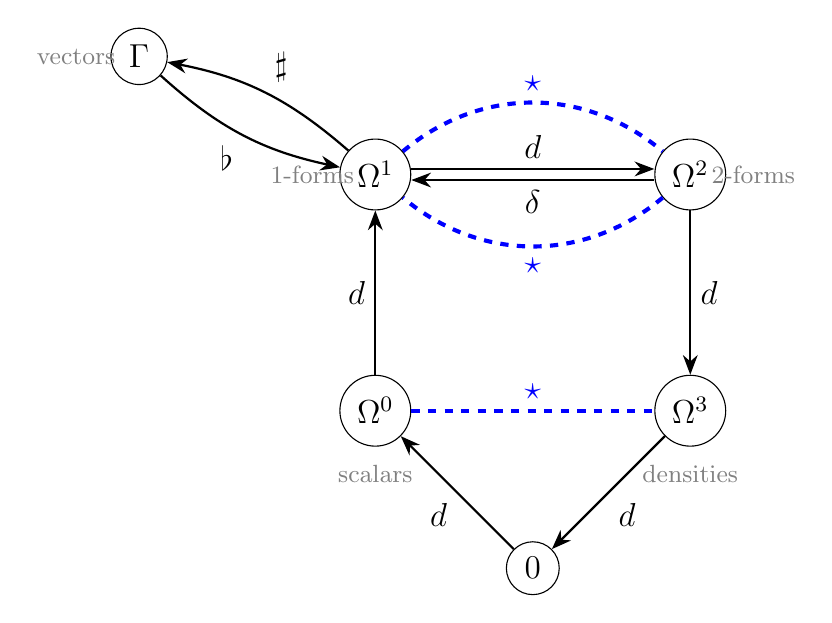
\begin{tikzpicture}[
    node distance=2.5cm and 3cm,
    every node/.style={font=\large},
    arrow/.style={-{Stealth[length=2.5mm]}, thick},
    hodge/.style={blue, dashed, line width=1.5pt},
    parallel shift/.style={transform canvas={yshift=#1}}
]

% === NODES ===
\node [draw, circle] (zero) at (0,-3.5) {$0$};
\node [draw, circle] (omega0) at (-2, -1.5) {$\Omega^0$};
\node [draw, circle] (omega3) at (2, -1.5) {$\Omega^3$};
\node [draw, circle] (omega1) at (-2, 1.5) {$\Omega^1$};
\node [draw, circle] (omega2) at (2, 1.5) {$\Omega^2$};
\node [draw, circle] (Gamma) at (-5, 3) {$\Gamma$};

% === DE RHAM COMPLEX ARROWS (d) ===
\draw[arrow] (zero) -- node[midway, below left] {$d$} (omega0);
\draw[arrow] (omega0) -- node[midway, left] {$d$} (omega1);
\draw[arrow, parallel shift=2pt] (omega1) -- node[midway, above] {$d$} (omega2);
\draw[arrow, parallel shift=-2pt] (omega2) -- node[midway, below] {$\delta$} (omega1);
\draw[arrow] (omega2) -- node[midway, right] {$d$} (omega3);
\draw[arrow] (omega3) -- node[midway, below right] {$d$} (zero);

% === HODGE STAR ARROWS ===
\draw[hodge] (omega0) -- node[midway, above] {$\star$} (omega3);
\draw[hodge, bend left=40] (omega1) to node[midway, above] {$\star$} (omega2);
\draw[hodge, bend left=40] (omega2) to node[midway, below] {$\star$} (omega1);

% === MUSICAL ISOMORPHISMS ===
\draw[-{Stealth[length=2.5mm]}, thick, bend right=15] 
    (Gamma) to node[midway, below left] {$\flat$} (omega1);
\draw[-{Stealth[length=2.5mm]}, thick, bend right=15] 
    (omega1) to node[midway, above right] {$\sharp$} (Gamma);

% === LABELS ===
\node[text=gray, font=\small] at (-2, -2.3) {scalars};
\node[text=gray, font=\small] at (2, -2.3) {densities};
\node[text=gray, font=\small] at (-2.8, 1.5) {1-forms};
\node[text=gray, font=\small] at (2.8, 1.5) {2-forms};
\node[text=gray, font=\small] at (-5.8, 3) {vectors};

\end{tikzpicture}
\end{center}

\begin{hott_commentary}[The Diamond as a Higher Inductive Type]
The Hodge--de Rham diamond can be formalized as a \emph{higher inductive type} (HIT) in HoTT. Define the type $\mathsf{Diamond}_3$ with:

\textbf{Point constructors}:
\begin{itemize}
\item $\Omega^k : \mathsf{Diamond}_3$ for $k \in \{0,1,2,3\}$
\item $\Gamma : \mathsf{Diamond}_3$ (vector fields)
\item $0 : \mathsf{Diamond}_3$ (trivial space)
\end{itemize}

\textbf{Path constructors}:
\begin{itemize}
\item $d_k : \Omega^k = \Omega^{k+1}$ (exterior derivative)
\item $\star_k : \Omega^k = \Omega^{3-k}$ (Hodge duality)
\item $\flat : \Gamma = \Omega^1$ and $\sharp : \Omega^1 = \Gamma$ (musical isomorphisms)
\end{itemize}

\textbf{2-path constructors} (coherences):
\begin{itemize}
\item $d^2 : d_{k+1} \circ d_k = \refl_{\Omega^{k+2}}$ (boundary of boundary is trivial)
\item $\star^2 : \star_{3-k} \circ \star_k = \pm\refl_{\Omega^k}$ (involutivity)
\item $\sharp\flat : \sharp \circ \flat = \refl_\Gamma$ and $\flat\sharp : \flat \circ \sharp = \refl_{\Omega^1}$
\end{itemize}

The \emph{univalence axiom} ensures that these path constructors (equivalences) can be treated as genuine identifications between spaces.
\end{hott_commentary}

\begin{categorical_commentary}[The Diamond as a 2-Category]
The Hodge--de Rham diamond is naturally a \emph{2-category} $\mathcal{D}_3$:
\begin{itemize}
\item \textbf{Objects}: The spaces $0, \Omega^0, \Omega^1, \Omega^2, \Omega^3, \Gamma$
\item \textbf{1-morphisms}: Linear maps $d, \delta, \star, \flat, \sharp$ and their composites
\item \textbf{2-morphisms}: Natural transformations expressing relations like $d^2 = 0$
\end{itemize}

The diagram satisfies several \emph{coherence conditions}:
\begin{enumerate}
\item The composite $d \circ d$ factors through the zero object (exactness).
\item The Hodge star satisfies $\star \circ d = \pm\delta \circ \star$ (intertwining).
\item Musical isomorphisms give an adjoint equivalence $\Gamma \simeq \Omega^1$.
\end{enumerate}

This 2-categorical structure is an instance of a \emph{Calabi--Yau $A_\infty$-category}, with the Hodge star providing the Calabi--Yau structure (a non-degenerate pairing).
\end{categorical_commentary}

\begin{qit_commentary}[The Diamond as a Quantum Circuit]
The Hodge--de Rham diamond can be interpreted as a \emph{quantum circuit diagram}:

\begin{itemize}
\item \textbf{Wires} ($\Omega^k$): Hilbert spaces carrying quantum states (forms)
\item \textbf{Gates}: 
\begin{itemize}
\item $d$ (exterior derivative): creation operator, adds a ``particle''
\item $\delta$ (codifferential): annihilation operator, removes a ``particle''
\item $\star$ (Hodge star): unitary transformation, ``Fourier transform''
\item $\flat, \sharp$: change of basis between ``position'' and ``velocity'' representations
\end{itemize}
\end{itemize}

The constraint $d^2 = 0$ is a \emph{supersymmetry constraint}: applying the creation operator twice annihilates the state. This is the hallmark of \emph{fermionic} systems---differential forms are the ``fermions'' of geometry.

The Hodge--Laplacian $\Delta = d\delta + \delta d$ is the \emph{Hamiltonian} of this supersymmetric quantum mechanics, and harmonic forms are \emph{BPS states} (annihilated by both supercharges $d$ and $\delta$).
\end{qit_commentary}

\subsection{Vector Calculus in Disguise}

The de Rham complex on $\mathbb{R}^3$, when translated through the metric isomorphisms, becomes the familiar sequence of vector calculus:
\[
0 \longrightarrow C^\infty(\mathbb{R}^3) \xrightarrow{\nabla} \mathfrak{X}(\mathbb{R}^3) \xrightarrow{\nabla\times} \mathfrak{X}(\mathbb{R}^3) \xrightarrow{\nabla\cdot} C^\infty(\mathbb{R}^3) \longrightarrow 0.
\]

The identities $\mathrm{curl} \circ \mathrm{grad} = 0$ and $\mathrm{div} \circ \mathrm{curl} = 0$ are simply the statement $d^2 = 0$.

\begin{ncg_commentary}[Vector Calculus from Spectral Data]
The spectral triple for $\mathbb{R}^3$ is $(C^\infty_c(\mathbb{R}^3), L^2(\mathbb{R}^3, \CC^2), D)$, where $D = -i\sigma^j \partial_j$ is the Dirac operator (with Pauli matrices $\sigma^j$).

The vector calculus operators emerge as:
\begin{align*}
\nabla f &= [D, f] \cdot e_j \quad \text{(gradient from commutator)} \\
\nabla \times \vec{v} &= \frac{1}{2}\epsilon^{ijk}\{[D, v_j], [D, v_k]\} \quad \text{(curl from anticommutator)} \\
\nabla \cdot \vec{v} &= \Tr([D, v_j] \cdot \gamma^j) \quad \text{(divergence from trace)}
\end{align*}

The identities $\nabla \times \nabla f = 0$ and $\nabla \cdot (\nabla \times \vec{v}) = 0$ follow from the \emph{Jacobi identity} for commutators and the \emph{cyclic property} of the trace.

This reformulation makes clear that vector calculus is a \emph{shadow} of Clifford algebra structure---a fact that becomes crucial for generalizations to curved and noncommutative spaces.
\end{ncg_commentary}

%=============================================================================
% SECTION 3: THE CLIFFORD BUNDLE
%=============================================================================
\section{The Clifford Bundle Formalism}\label{sec:clifford}

\subsection{Definition of the Clifford Bundle}

\begin{definition}[Clifford Bundle]
Let $(M,g)$ be a (pseudo-)Riemannian manifold. The \textbf{Clifford bundle} $\mathcal{C}\ell(M,g)$ is the vector bundle whose fiber at each point $x \in M$ is the Clifford algebra $\mathcal{C}\ell(T_xM, g_x)$:
\[
\mathcal{C}\ell(M,g) = \frac{\bigoplus_{k=0}^{\infty} T^{(k)}M}{\langle v \otimes v - g(v,v) \cdot 1 \rangle}
\]
where the ideal imposes the \textbf{Clifford relation} $v \cdot v = g(v,v)$.
\end{definition}

A section $\psi \in \Gamma(\mathcal{C}\ell(M,g))$ expands locally as:
\[
\psi(x) = f(x) + v^i(x)e_i + \tfrac{1}{2!}F^{ij}(x)e_i \wedge e_j + \tfrac{1}{3!}T^{ijk}(x)e_i \wedge e_j \wedge e_k + \cdots
\]
where $\{e_i\}$ is a local orthonormal frame for $TM$ and the coefficients are smooth functions.

\begin{hott_commentary}[The Clifford Algebra as a Quotient Type]
In HoTT, the Clifford algebra $\mathcal{C}\ell(V,q)$ is constructed as a \emph{quotient type}:
\[
\mathcal{C}\ell(V,q) := T(V) / \sim
\]
where $T(V) = \bigoplus_{k=0}^\infty V^{\otimes k}$ is the tensor algebra (an inductive type) and $\sim$ is the equivalence relation generated by $v \otimes v \sim q(v) \cdot 1$.

The quotient is defined as a \emph{higher inductive type}:
\begin{itemize}
\item \textbf{Point constructor}: $[-] : T(V) \to \mathcal{C}\ell(V,q)$
\item \textbf{Path constructor}: For all $v \in V$, $\mathsf{cliff}_v : [v \otimes v] = [q(v) \cdot 1]$
\item \textbf{Set-truncation}: $\mathcal{C}\ell(V,q)$ is a 0-type (set)
\end{itemize}

The \emph{universal property} states that any linear map $f: V \to A$ to an algebra $A$ satisfying $f(v)^2 = q(v) \cdot 1_A$ extends uniquely to an algebra homomorphism $\tilde{f}: \mathcal{C}\ell(V,q) \to A$.

This universal property is the type-theoretic expression of the fact that Clifford algebras are ``initial'' among algebras with the Clifford relation.
\end{hott_commentary}

\begin{categorical_commentary}[The Clifford Functor]
The construction of Clifford algebras is \emph{functorial}. Define the category $\mathsf{Quad}$ of quadratic spaces $(V,q)$ with isometries as morphisms. The Clifford algebra defines a functor:
\[
\mathcal{C}\ell : \mathsf{Quad} \to \mathsf{Alg}_\RR
\]
This functor is the \emph{left adjoint} to the forgetful functor $U: \mathsf{Alg}_\RR \to \mathsf{Quad}$ sending an algebra $A$ to its underlying vector space with the quadratic form $q(a) = a^2$:
\[
\mathcal{C}\ell \dashv U
\]

For vector bundles, this extends to a functor:
\[
\mathcal{C}\ell : \mathsf{Riem} \to \mathsf{AlgBun}
\]
from Riemannian manifolds to algebra bundles. The Clifford bundle $\mathcal{C}\ell(M,g)$ is the value of this functor on $(M,g)$.

The grading $\mathcal{C}\ell = \mathcal{C}\ell^{\mathrm{even}} \oplus \mathcal{C}\ell^{\mathrm{odd}}$ makes $\mathcal{C}\ell$ a \emph{superalgebra}, and the functor lands in the category $\mathsf{SuperAlg}$.
\end{categorical_commentary}

\begin{ncg_commentary}[Clifford Algebras and K-Theory]
The Clifford algebras exhibit \emph{Bott periodicity}:
\[
\mathcal{C}\ell(p+8, q) \cong \mathcal{C}\ell(p,q) \otimes \mathcal{C}\ell(8,0) \cong \mathcal{C}\ell(p,q) \otimes \mathrm{Mat}_{16}(\RR)
\]
This 8-fold periodicity is the \emph{real Bott periodicity} for KO-theory.

In Connes' framework, the \emph{KO-dimension} of a spectral triple $(A,H,D)$ is determined by the signs $(\epsilon, \epsilon', \epsilon'')$ in the relations:
\[
J^2 = \epsilon, \quad JD = \epsilon' DJ, \quad J\gamma = \epsilon'' \gamma J
\]
These signs repeat with period 8 as a function of dimension, reflecting the Clifford periodicity.

The physical consequence is that \emph{fermion chirality, charge conjugation, and dimension} are interrelated through the Clifford algebra structure---the Standard Model particle content is constrained by KO-dimension 6 (or equivalently, dimension 10 for the full spacetime).
\end{ncg_commentary}

\begin{qit_commentary}[Clifford Algebras as Fermionic Systems]
In quantum information, Clifford algebras describe \emph{fermionic quantum systems}. The generators $e_1, \ldots, e_n$ of $\mathcal{C}\ell(n,0)$ satisfy:
\[
e_i e_j + e_j e_i = 2\delta_{ij}
\]
which are the \emph{canonical anticommutation relations} (CAR) for $n$ fermionic modes.

The Clifford algebra $\mathcal{C}\ell(2n,0) \cong \mathrm{Mat}_{2^n}(\CC)$ acts on the \emph{Fock space} $\mathcal{F} = \bigwedge \CC^n$ of $n$ fermions, with:
\begin{align*}
c_j &= e_{2j-1} + ie_{2j} \quad \text{(annihilation operator)} \\
c_j^\dagger &= e_{2j-1} - ie_{2j} \quad \text{(creation operator)}
\end{align*}

The \emph{Clifford group} $\mathrm{Pin}(n) \subset \mathcal{C}\ell(n,0)^\times$ acts on fermions by \emph{Bogoliubov transformations}, and the spin representation is the \emph{particle number parity} grading.

Differential forms on a manifold are thus ``fermions living on spacetime,'' with the exterior derivative as the Dirac operator coupling them to geometry.
\end{qit_commentary}

\subsection{Physical Correspondence by Grade}

Sections of $\mathcal{C}\ell(M,g)$ are \textbf{multivector fields}, unifying different geometric and physical objects:

\begin{center}
\renewcommand{\arraystretch}{1.4}
\begin{tabular}{c >{\raggedright}p{3.5cm} p{8.5cm}}
\toprule
\textbf{Grade} & \textbf{Mathematical Object} & \textbf{Physical Examples} \\
\midrule
0 & Scalar field & Higgs field $\phi$, dilaton, cosmological constant $\Lambda$, wave function amplitude \\
1 & Vector field / 1-form & 4-potential $A_\mu$, momentum $p_\mu$, current density $j^\mu$, velocity field \\
2 & Bivector / 2-form & Electromagnetic field $F_{\mu\nu}$, angular momentum $L_{\mu\nu}$, Riemann curvature \\
3 & Trivector / 3-form & Torsion $T_{\mu\nu\rho}$, M-theory C-field $C_{\mu\nu\rho}$, Hodge dual of current \\
4 & Pseudoscalar / 4-form & Volume form $\epsilon_{\mu\nu\rho\sigma}$, axion field, $\theta$-term in QCD, chirality operator $\gamma^5$ \\
\bottomrule
\end{tabular}
\end{center}

\begin{qit_commentary}[Grades as Particle Number]
The grading of multivector fields corresponds to \emph{particle number} in the fermionic Fock space interpretation:
\begin{itemize}
\item Grade 0: vacuum state $|0\rangle$
\item Grade 1: single-particle states $c_i^\dagger |0\rangle$
\item Grade 2: two-particle states $c_i^\dagger c_j^\dagger |0\rangle$
\item Grade $k$: $k$-particle states
\end{itemize}

The exterior derivative $d$ acts as a \emph{single-particle excitation operator}, and the condition $d^2 = 0$ is the \emph{Pauli exclusion principle}---you cannot create the same fermion twice.

The electromagnetic field $F \in \Omega^2$ is a ``two-fermion'' state, explaining why photons (despite being bosons) arise from a 2-form: they are \emph{bound states of two form-fermions}, analogous to Cooper pairs in superconductivity.
\end{qit_commentary}

\subsection{Unified Operators and Field Equations}

The Clifford bundle formalism allows fundamental field equations to be written in remarkably unified forms.

\subsubsection{The Dirac--de Rham Operator}

The \textbf{geometric derivative} $D = d + \delta$ unifies the exterior derivative and codifferential:
\[
D^2 = (d + \delta)^2 = d\delta + \delta d = \Delta \qquad \text{(Hodge--Laplacian)}
\]

\begin{ncg_commentary}[The Dirac Operator as Fundamental]
In noncommutative geometry, the Dirac operator $D$ is the \emph{fundamental datum}---more fundamental than the metric, which is recovered from it.

\textbf{Connes' reconstruction theorem} states that for a commutative spectral triple $(C^\infty(M), L^2(S), D)$ satisfying certain axioms, the manifold $M$ and metric $g$ can be recovered from the spectrum of $D$ alone:
\[
g_{\mu\nu}(x) = \lim_{t \to 0} t \cdot \Tr(\gamma_\mu [D, x^\nu] e^{-tD^2})
\]

The de Rham--Dirac operator $D = d + \delta$ (acting on forms) is related to the spinor Dirac operator by:
\[
D_{\text{forms}}^2 = D_{\text{spinor}}^2 \quad \text{(Lichnerowicz formula)}
\]
Both encode the same geometric information---the metric and curvature.

For noncommutative spaces (e.g., the Standard Model as a product $M \times F$ of spacetime with a finite internal space), the Dirac operator encodes both gravitational and gauge degrees of freedom. The Higgs field emerges as the ``connection 1-form'' on the internal space.
\end{ncg_commentary}

\subsubsection{Maxwell's Equations}

In the Clifford formalism, Maxwell's four equations collapse to one:
\[
\boxed{\nabla F = J}
\]
where $F = \mathbf{E} + I\mathbf{B} \in \Gamma(\mathcal{C}\ell(M,g))$ is a bivector field, $J = \rho - \mathbf{j}$ is a vector field, $\nabla = \gamma^\mu \partial_\mu$ is the vector derivative, and $I$ is the pseudoscalar unit.

\begin{hott_commentary}[Maxwell's Equations as a Fiber Sequence]
In HoTT, Maxwell's equations $\nabla F = J$ can be interpreted as a statement about a \emph{fiber sequence} of types:
\[
\Omega^0 \xrightarrow{d} \Omega^1 \xrightarrow{d} \Omega^2 \xrightarrow{d} \Omega^3
\]

The electromagnetic potential $A \in \Omega^1$ is a \emph{path} in gauge space, and the field strength $F = dA \in \Omega^2$ is the \emph{curvature} of this path. The Bianchi identity $dF = 0$ states that ``the curvature of curvature is trivial''---an identity type at the level of 3-cells.

The equation $d\star F = J$ (Gauss's law and Ampère's law) is a statement that the \emph{codifferential} of $F$ equals the current, which in type-theoretic terms asserts a \emph{section} of a certain fibration.

Gauge transformations $A \mapsto A + d\lambda$ are \emph{homotopies} between paths, and physically equivalent configurations are identified by the univalence axiom.
\end{hott_commentary}

\subsubsection{The Dirac Equation}

The Dirac equation in Clifford form:
\[
\nabla \psi I \sigma_3 - eA \psi = m \psi \gamma_0
\]
where $\psi \in \Gamma(\mathcal{C}\ell(M,g))$ is an even multivector representing the Dirac spinor.

\begin{qit_commentary}[The Dirac Equation as a Quantum Walk]
The Dirac equation can be discretized into a \emph{quantum walk}---a quantum analog of a random walk where the walker moves in superposition.

The Dirac operator $D = \sum_\mu \gamma^\mu \partial_\mu$ is a sum of \emph{shift operators} (translations in each direction) weighted by \emph{coin operators} (the gamma matrices):
\[
e^{-itD} = \lim_{N\to\infty} \left(\prod_\mu e^{-i\frac{t}{N}\gamma^\mu \partial_\mu}\right)^N
\]

This is the basis for \emph{lattice fermion simulations} and has been proposed for \emph{quantum simulation of high-energy physics} on quantum computers.

The Clifford algebra structure ensures that the quantum walk has the correct \emph{relativistic dispersion relation} $E^2 = p^2 + m^2$, with the gamma matrices encoding the ``internal coin space'' of the walker.
\end{qit_commentary}

\subsection{Advantages of the Clifford Bundle Formalism}

\begin{enumerate}
\item \textbf{Coordinate Independence}: Physical laws are manifestly coordinate-free and geometric.

\item \textbf{Unification of Algebra and Geometry}: The Clifford product combines wedge (geometry) and inner (metric) products.

\item \textbf{Spinors as Minimal Ideals}: Spinor fields emerge naturally as minimal left ideals of the Clifford algebra.

\item \textbf{Computational Efficiency}: Often simplifies calculations in relativistic physics and general relativity.

\item \textbf{Quantum--Classical Bridge}: The same framework describes classical fields (multivectors) and quantum fields (spinor representations).
\end{enumerate}

\begin{categorical_commentary}[The Clifford Bundle as a Monoidal Category]
The Clifford bundle has rich categorical structure. Consider the category $\mathcal{C}\ell\text{-}\mathsf{Mod}$ of $\mathcal{C}\ell(M,g)$-modules (vector bundles with Clifford action):

\begin{enumerate}
\item It is a \emph{monoidal category} under the graded tensor product $\otimes_{\mathcal{C}\ell}$.

\item It has a \emph{dagger structure} from the Clifford involution $v \mapsto -v$, making it a $\dagger$-category.

\item The \emph{spinor bundle} $S$ is a \emph{simple object}---it cannot be decomposed into smaller Clifford modules.

\item \emph{Morita equivalence}: $\mathcal{C}\ell(p,q)$ and $\mathcal{C}\ell(p',q')$ have equivalent module categories iff $(p-q) \equiv (p'-q') \mod 8$ (another manifestation of Bott periodicity).
\end{enumerate}

The physical interpretation is that particle types (representations of $\mathrm{Spin}(p,q)$) are organized by the \emph{Morita class} of the Clifford algebra, which depends only on signature mod 8.
\end{categorical_commentary}

%=============================================================================
% SECTION 4: THE CENTRALITY OF Ω²
%=============================================================================
\section{The Centrality of $\Omega^2$: The Dynamics Level}\label{sec:omega2}

\subsection{Why 2-Forms Are Central}

Placing $\Omega^2$ at the geometric center of the diagram reveals deep physical significance.

\subsubsection{Field Strength Lives in $\Omega^2$}

In gauge theory, the hierarchy is:
\[
\underbrace{\Omega^0}_{\text{gauge function}} \xrightarrow{d} 
\underbrace{\Omega^1}_{\text{potential } A} \xrightarrow{d} 
\underbrace{\Omega^2}_{\text{field strength } F} \xrightarrow{d} 
\underbrace{\Omega^3}_{\text{Bianchi } dF=0}
\]

The physics (energy, equations of motion, observables) lives at $\Omega^2$:
\begin{itemize}
\item Electromagnetic field: $F = dA \in \Omega^2$
\item Yang--Mills curvature: $F = dA + A \wedge A \in \Omega^2$
\item Riemann curvature: $R^a{}_b \in \Omega^2(\mathfrak{so}(n))$
\end{itemize}

\begin{hott_commentary}[Curvature as Holonomy]
In HoTT, the curvature 2-form $F$ encodes \emph{holonomy}---the failure of parallel transport around loops to be trivial.

Consider a principal $G$-bundle $P \to M$. A connection $A$ assigns to each path $\gamma: x \to y$ a group element $\mathrm{hol}_A(\gamma) \in G$ (the holonomy). For a contractible loop $\gamma: x \to x$, we might expect $\mathrm{hol}_A(\gamma) = 1_G$, but this fails when curvature is present:
\[
\mathrm{hol}_A(\partial \Sigma) = \mathcal{P}\exp\left(\int_\Sigma F\right) \neq 1_G
\]

In type-theoretic terms, the curvature measures the \emph{obstruction to extending a section} from the 1-skeleton to the 2-skeleton. This is a \emph{cohomological} statement: $F$ represents a class in $H^2(M; \mathfrak{g})$.

The centrality of $\Omega^2$ reflects the fact that \emph{2-cells are where topology lives}---fundamental groups detect 1-holes, but interesting physics (instantons, monopoles) lives in the interaction between 1-forms and 2-forms.
\end{hott_commentary}

\begin{remark}[Emergent Complex Structure]
The Hodge star $\star$ acts as a complex structure ($J$) on $\Omega^2$ in Minkowski space because $\star^2 = -1$ on 2-forms. This explains why complex numbers appear naturally in physics---they are an emergent property of the geometry of 2-forms.
\end{remark}

\begin{ncg_commentary}[The Spectral Action on $\Omega^2$]
In Connes' \emph{spectral action principle}, the dynamics of gauge fields arises from:
\[
S = \Tr(f(D/\Lambda))
\]
where $f$ is a cutoff function and $\Lambda$ is an energy scale. Expanding this for small $D/\Lambda$ yields:
\[
S = \int_M \left( c_0 + c_1 R + c_2 |F|^2 + \cdots \right) \sqrt{g} \, d^4x
\]
where $R$ is scalar curvature and $|F|^2$ is the Yang--Mills action.

The gauge field strength $F \in \Omega^2$ appears at the \emph{second order} in this expansion---confirming that $\Omega^2$ is the ``dynamics level.'' Higher-order terms involve curvatures (also 2-forms) contracted in various ways.

The spectral action thus \emph{derives} the centrality of $\Omega^2$ from the spectrum of the Dirac operator: field strengths are the leading non-topological contribution to the action.
\end{ncg_commentary}

\begin{qit_commentary}[2-Forms as Entanglement]
In quantum information, 2-forms have an interpretation as \emph{entanglement} between subsystems.

Consider a bipartite system with subsystems $A$ and $B$. The state space is $\mathcal{H}_A \otimes \mathcal{H}_B$. A 2-form $\omega \in \Omega^1_A \wedge \Omega^1_B$ encodes correlations between the two subsystems:
\[
\omega = \sum_{i,j} \omega_{ij} \, dx^i \wedge dy^j
\]
where $x^i$ are coordinates on $A$ and $y^j$ on $B$.

The \emph{self-duality} condition $\star \omega = \pm i\omega$ (in 4D with Lorentzian signature) corresponds to \emph{maximal entanglement}---states that are eigenstates of the partial transpose.

This interpretation extends to gauge theory: the field strength $F$ encodes ``entanglement between points of spacetime,'' mediated by the gauge field. Instantons (self-dual $F$) represent \emph{maximally entangled} configurations of the gauge field.
\end{qit_commentary}

%=============================================================================
% SECTION 5: MINKOWSKI SPACE
%=============================================================================
\section{The Hodge--de Rham Complex in Minkowski Space}\label{sec:minkowski}

\subsection{The Extended Diamond in 4D}

For Minkowski space $\mathbb{R}^{3,1}$ with signature $(+,+,+,-)$, the de Rham complex extends to:
\[
0 \to \Omega^0 \xrightarrow{d} \Omega^1 \xrightarrow{d} \Omega^2 \xrightarrow{d} \Omega^3 \xrightarrow{d} \Omega^4 \to 0
\]

The Hodge star satisfies $\star^2 = (-1)^{k(4-k)+1}$ on $k$-forms:
\begin{itemize}
\item $\Omega^0 \xleftrightarrow{\star} \Omega^4$: $\star^2 = -1$
\item $\Omega^1 \xleftrightarrow{\star} \Omega^3$: $\star^2 = +1$
\item $\Omega^2 \xrightarrow{\star} \Omega^2$: $\star^2 = -1$ (complex structure)
\end{itemize}

\begin{categorical_commentary}[The Lorentzian Diamond as a Dagger Category]
The Lorentzian signature introduces subtle categorical structure. The Hodge star $\star: \Omega^k \to \Omega^{4-k}$ satisfies:
\begin{itemize}
\item $\star^2 = (-1)^s$ where $s$ depends on $k$ and signature
\item $\star$ is an \emph{antilinear} involution when complexified
\end{itemize}

This makes the complexified de Rham complex a \emph{$\dagger$-category}, where the dagger is $\dagger = \star \circ \overline{(\cdot)}$ (Hodge star composed with complex conjugation).

The \emph{unitarity} condition $\omega^\dagger = \omega$ picks out \emph{real} forms, while $\omega^\dagger = -\omega$ picks out \emph{imaginary} forms. The self-dual forms $F_+ = \frac{1}{2}(F - i\star F)$ satisfy $F_+^\dagger = F_-$, showing that self-duality mixes with the $\dagger$-structure.

This categorical perspective explains why \emph{Wick rotation} (Euclidean signature) is needed for rigorous QFT: it makes $\star^2 = +1$ on 2-forms, so $\star$ becomes a genuine involution (not a complex structure), and the path integral is well-defined.
\end{categorical_commentary}

\subsection{Self-Duality and Instantons}

Since $\star^2 = -1$ on 2-forms, we define complex self-dual and anti-self-dual parts:
\[
F_{\pm} = \frac{1}{2}(F \mp i\star F), \qquad \star F_{\pm} = \pm i F_{\pm}.
\]
This decomposition is fundamental to:
\begin{itemize}
\item Instantons in Yang--Mills theory ($F = \star F$ becomes $F_- = 0$)
\item Twistor theory and the Penrose transform
\item Chiral representations of the Lorentz group
\item Maxwell's equations in vacuum: $dF = 0$ and $d\star F = 0$ imply $dF_{\pm} = 0$
\end{itemize}

\begin{hott_commentary}[Self-Duality and Univalence]
The self-duality condition $F = \star F$ can be understood type-theoretically through the \emph{univalence axiom}.

The Hodge star defines an \emph{equivalence} $\star: \Omega^2 \simeq \Omega^2$. By univalence, this corresponds to a \emph{path} in the universe:
\[
\ua(\star) : \Omega^2 =_{\Type} \Omega^2
\]

A self-dual form $F$ satisfies $F = \star F$, which means $F$ is a \emph{fixed point} of the equivalence $\star$. The space of such fixed points is:
\[
\Omega^2_+ = \{F : \Omega^2 \mid F = \star F\} = \sum_{F:\Omega^2} (F =_{\Omega^2} \star F)
\]

By the path induction principle, this space is non-trivial only when $\star$ has fixed points---which requires $\star^2 = \Id$ (up to homotopy). In Lorentzian signature, $\star^2 = -1$, so there are no \emph{real} fixed points, but \emph{complex} fixed points exist (using the complex structure $i$ with $i^2 = -1$).

This type-theoretic analysis reveals that \emph{instantons exist only upon complexification}---a fact with profound physical consequences for quantum Yang--Mills theory.
\end{hott_commentary}

\begin{qit_commentary}[Self-Duality and Quantum Error Correction]
Self-dual codes in quantum error correction are the analog of self-dual forms.

A \emph{stabilizer code} is defined by a subgroup $S \subset \mathcal{P}_n$ of the Pauli group. The code is \emph{self-dual} if $S = S^\perp$ (the code equals its symplectic complement).

The connection to forms: the Pauli group on $n$ qubits is $\mathcal{P}_n \cong \ZZ_2^{2n}$, which can be identified with the ``discrete 1-forms'' on a lattice. The stabilizer subgroup $S$ is a ``discrete 2-form'' (via the boundary map $\partial: C_2 \to C_1$), and self-duality is exactly the condition $S = \star S$ where $\star$ is the symplectic form on $\ZZ_2^{2n}$.

Famous self-dual codes include the \emph{toric code} (a lattice discretization of a self-dual gauge theory) and the \emph{color code}. The \emph{self-duality} of these codes is inherited from the Hodge duality of the underlying geometric structure.
\end{qit_commentary}

%=============================================================================
% SECTION 6: THE OCTONIONIC EXTENSION
%=============================================================================
\section{The Octonionic Hodge--de Rham Complex}\label{sec:octonionic}

\subsection{The Special Status of 7 Dimensions}

The Hodge--de Rham complex for the Clifford algebra $\mathrm{Cl}(0,7)$ represents one of the most physically rich structures in modern theoretical physics. Seven dimensions hold a privileged position because of the connection to octonions and $G_2$ holonomy.

\begin{hott_commentary}[Octonions and Higher Structure]
The octonions $\OO$ are the largest normed division algebra, but they are \emph{non-associative}: $(xy)z \neq x(yz)$ in general.

In HoTT, non-associativity manifests as \emph{higher coherence data}. For an associative algebra, we have a path:
\[
\alpha_{x,y,z} : (xy)z = x(yz)
\]
For octonions, this path \emph{does not exist} in general. Instead, we have the \emph{alternativity} conditions:
\[
x(xy) = (xx)y, \qquad (yx)x = y(xx)
\]
which provide weaker coherences.

The \emph{automorphism group} $\mathrm{Aut}(\OO) = G_2$ is the exceptional Lie group preserving the octonionic multiplication. In type-theoretic terms, $G_2$ is the space of \emph{auto-equivalences} of the octonionic type that respect the multiplication:
\[
G_2 = \{g : \OO \simeq \OO \mid g(xy) = g(x)g(y)\}
\]

The 7-dimensional imaginary octonions $\mathrm{Im}(\OO)$ carry a $G_2$-structure, and the Hodge--de Rham complex on a 7-manifold with $G_2$ holonomy inherits this non-associative structure via the \emph{associative 3-form}.
\end{hott_commentary}

\subsubsection{$G_2$ as the Smallest Exceptional Lie Group}

The exceptional Lie group $G_2 \subset \mathrm{SO}(7)$ with $\dim(G_2) = 14$ preserves the octonionic structure and decomposes the form spaces:
\begin{align*}
\Omega^1(\mathbb{R}^7) &= \Lambda^1_7 &&\text{(fundamental representation)} \\
\Omega^2(\mathbb{R}^7) &= \Lambda^2_7 \oplus \Lambda^2_{14} &&\text{where } \Lambda^2_{14} \cong \mathfrak{g}_2 \\
\Omega^3(\mathbb{R}^7) &= \Lambda^3_1 \oplus \Lambda^3_7 \oplus \Lambda^3_{27}
\end{align*}

\begin{categorical_commentary}[$G_2$ as an Automorphism 2-Group]
The group $G_2$ has a rich categorical interpretation. It is the automorphism group of several exceptional structures:

\begin{enumerate}
\item $G_2 = \mathrm{Aut}(\OO)$ (octonion automorphisms)
\item $G_2 = \mathrm{Stab}_{SO(7)}(\varphi)$ (stabilizer of the associative 3-form)
\item $G_2 = \mathrm{Aut}(\mathrm{Fano})$ (automorphisms of the Fano plane, the projective plane over $\mathbb{F}_2$)
\end{enumerate}

These different characterizations are related by \emph{Tannaka duality}: $G_2$ is determined by its representation category $\mathsf{Rep}(G_2)$, which is a \emph{braided monoidal category} with exceptional fusion rules.

The representations of $G_2$ are indexed by pairs of non-negative integers $(a,b)$ with dimensions:
\[
\dim V_{(a,b)} = \frac{(a+1)(b+1)(a+b+2)(a+2b+3)(2a+b+3)(a+b+3)}{360}
\]
The fundamental representations are $V_{(1,0)} = \mathbf{7}$ and $V_{(0,1)} = \mathbf{14} = \mathfrak{g}_2$.

This representation-theoretic structure constrains what fields can propagate on a $G_2$ manifold.
\end{categorical_commentary}

\subsection{The Associative and Coassociative Forms}

\subsubsection{The Associative 3-Form $\varphi$}

Defined by octonion multiplication:
\[
\varphi_{ijk} = \langle e_i \times_{\mathbb{O}} e_j, e_k \rangle
\]
This form encodes:
\begin{itemize}
\item $G_2$ structure on 7-manifolds
\item Calibrations for minimal submanifolds
\item Torsion-free condition: $d\varphi = 0$ and $d\star\varphi = 0$ defines $G_2$ holonomy
\end{itemize}

\begin{ncg_commentary}[The $G_2$ Spectral Triple]
A 7-manifold $X$ with $G_2$ holonomy admits a spectral triple $(C^\infty(X), L^2(S), D)$ with special properties:

\begin{enumerate}
\item The spinor bundle $S$ is 8-dimensional (real), matching the dimension of $\OO$.
\item The Dirac operator $D$ splits as $D = D_+ \oplus D_-$ under the triality decomposition.
\item The \emph{spectral action} on a $G_2$ manifold reduces to:
\[
S = \int_X \left( R - \frac{1}{2}|T|^2 + \cdots \right) \sqrt{g} \, d^7x
\]
where $T$ is the torsion of the $G_2$ structure.
\end{enumerate}

The torsion-free condition $d\varphi = d\star\varphi = 0$ is equivalent to \emph{Ricci-flatness} plus the constraint that the spinor covariant derivative of a certain parallel spinor vanishes. This makes $G_2$ manifolds the 7-dimensional analogs of Calabi--Yau manifolds.

In M-theory, compactification on a $G_2$ manifold preserves $\mathcal{N}=1$ supersymmetry in 4D, with the spectral triple encoding both the gravitational and matter sectors.
\end{ncg_commentary}

\subsubsection{The Coassociative 4-Form $\star\varphi$}

The Hodge dual satisfies the remarkable relation:
\[
\star\varphi = \frac{1}{2}\varphi \wedge \varphi
\]
This is crucial for topological field theory on $G_2$ manifolds, Donaldson--Thomas invariants, and M-theory.

\begin{qit_commentary}[$G_2$ and Quantum Error Correction]
The exceptional structure of $G_2$ manifests in quantum error-correcting codes.

The \emph{$[7,1,3]$ Hamming code} is a classical error-correcting code with 7 bits encoding 1 logical bit, correcting 1 error. Its automorphism group contains $\mathrm{PSL}(3,2) = \mathrm{GL}(3,\mathbb{F}_2)$, which acts on the Fano plane.

The quantum analog is the \emph{Steane code}, a $[[7,1,3]]$ CSS code. Its \emph{transversal gates} include the entire Clifford group, and it has a remarkable connection to $G_2$:
\begin{itemize}
\item The 7 physical qubits correspond to the 7 imaginary units of $\OO$.
\item The stabilizers correspond to the 7 ``associative triples'' in $\OO$ (lines in the Fano plane).
\item The logical operators correspond to $G_2$-invariant structures.
\end{itemize}

More generally, the exceptional Jordan algebra $\mathfrak{J}_3(\OO)$ encodes a \emph{27-dimensional code space} whose error-correcting properties are governed by $E_6$ (the automorphism group of the Jordan structure).
\end{qit_commentary}

\subsection{Octonionic Triality}

The triality of $\mathrm{Spin}(8)$:
\[
8_v \otimes 8_s \otimes 8_c \quad \text{with symmetry group } S_3
\]
where $8_v$, $8_s$, $8_c$ are vector, spinor, and conjugate spinor representations.

\begin{hott_commentary}[Triality as a 3-Fold Loop]
Triality is a symmetry that \emph{cyclically permutes} three representations of $\mathrm{Spin}(8)$. In HoTT, this is captured by a \emph{3-fold loop} in the universe.

Consider the type of 8-dimensional real representations:
\[
\mathsf{Rep}_8 = \sum_{V : \Type} \|V \simeq \RR^8\|
\]
Triality defines a \emph{path}:
\[
\tau : 8_v =_{\mathsf{Rep}_8} 8_s =_{\mathsf{Rep}_8} 8_c =_{\mathsf{Rep}_8} 8_v
\]
This is a \emph{non-trivial 3-loop}, corresponding to the outer automorphism of $\mathrm{Spin}(8)$ of order 3.

The existence of such a loop is highly exceptional: for $n \neq 8$, the only outer automorphisms of $\mathrm{Spin}(n)$ have order 2 (corresponding to charge conjugation). Triality is a ``third kind of duality'' that only exists in 8 dimensions.

Physical consequences:
\begin{itemize}
\item Type IIA, IIB, and heterotic strings are related by triality.
\item The three generations of fermions may be related to triality.
\item Exceptional holonomies ($G_2$, $\mathrm{Spin}(7)$) arise from breaking triality symmetry.
\end{itemize}
\end{hott_commentary}

\begin{categorical_commentary}[Triality as a 2-Categorical Structure]
Triality defines a \emph{2-group} structure on the Spin group. Consider the crossed module:
\[
1 \to \ZZ_3 \to \mathrm{Aut}(\mathrm{Spin}(8)) \to \mathrm{Out}(\mathrm{Spin}(8)) \to 1
\]
where $\mathrm{Out}(\mathrm{Spin}(8)) = S_3$ is the group of outer automorphisms (including triality).

This can be promoted to a \emph{2-group} $\mathbb{G}$:
\begin{itemize}
\item Objects: the identity
\item 1-morphisms: elements of $\mathrm{Out}(\mathrm{Spin}(8)) = S_3$
\item 2-morphisms: inner automorphisms relating different representatives
\end{itemize}

Principal $\mathbb{G}$-bundles classify ``triality-twisted'' Spin structures, which appear in:
\begin{itemize}
\item F-theory compactifications
\item Non-geometric string backgrounds
\item Exotic smooth structures on 4-manifolds
\end{itemize}

The categorical perspective reveals that triality is not just a group-theoretic curiosity but a \emph{2-categorical phenomenon} with physical consequences.
\end{categorical_commentary}

\subsection{Applications to M-Theory}

\subsubsection{M-Theory Compactifications}

Compactification of 11-dimensional supergravity on 7D $G_2$ holonomy manifolds preserves $\mathcal{N}=1$ supersymmetry in 4D:
\[
\text{M-theory on } \mathbb{R}^{1,3} \times X_{G_2} \to \mathcal{N}=1 \text{ supergravity in 4D}
\]

\begin{ncg_commentary}[M-Theory and Exceptional Noncommutative Geometry]
M-theory compactification on $G_2$ manifolds can be reformulated in the language of noncommutative geometry.

The internal space $X_{G_2}$ is encoded in a spectral triple $(A, H, D)$ where:
\begin{itemize}
\item $A = C^\infty(X_{G_2})$ is the algebra of smooth functions
\item $H = L^2(X_{G_2}, S)$ is the spinor Hilbert space
\item $D$ is the Dirac operator twisted by the $G_2$ structure
\end{itemize}

The \emph{spectral action}:
\[
S = \Tr(f(D/\Lambda)) + \langle J\Psi, D\Psi \rangle
\]
reproduces the 4D effective action including:
\begin{itemize}
\item Einstein--Hilbert gravity from the bosonic part
\item Gauge fields from the internal Dirac operator
\item Yukawa couplings from the fermionic part
\end{itemize}

For the Standard Model coupled to gravity, Connes and collaborators showed that the appropriate spectral triple has \emph{KO-dimension 6}, matching $M^4 \times X_6$ where $X_6$ is a ``finite noncommutative space'' encoding the gauge and Higgs sectors.

The $G_2$ manifold provides a \emph{geometric realization} of this finite space, with the exceptional structure of $G_2$ constraining the possible gauge groups and matter content.
\end{ncg_commentary}

%=============================================================================
% SECTION 7: THE EXCEPTIONAL JORDAN ALGEBRA
%=============================================================================
\section{The Exceptional Jordan Algebra and $E_8$}\label{sec:jordan}

\subsection{The Albert Algebra}

\begin{definition}[Albert Algebra]
The \textbf{exceptional Jordan algebra} $\mathfrak{J}_3(\mathbb{O})$ is the algebra of $3 \times 3$ Hermitian matrices over the octonions:
\[
\mathfrak{J}_3(\mathbb{O}) = \left\{ 
\begin{pmatrix}
a & x & \bar{y} \\
\bar{x} & b & z \\
y & \bar{z} & c
\end{pmatrix} : a,b,c \in \mathbb{R}, \; x,y,z \in \mathbb{O}
\right\}
\]
with Jordan product $X \circ Y = \frac{1}{2}(XY + YX)$.
\end{definition}

This 27-dimensional algebra possesses extraordinary properties:
\begin{itemize}
\item \textbf{Non-associative but power-associative}: $(A \circ B) \circ A^2 = A \circ (B \circ A^2)$
\item \textbf{Exceptional}: Cannot be realized as a subalgebra of an associative algebra
\item \textbf{Symmetry group}: Automorphism group is the exceptional Lie group $F_4$
\end{itemize}

\begin{hott_commentary}[The Albert Algebra as a Higher Algebraic Structure]
In HoTT, the Albert algebra presents a fascinating example of a \emph{higher algebraic structure} that cannot be reduced to associative operations.

A Jordan algebra satisfies:
\begin{enumerate}
\item Commutativity: $x \circ y = y \circ x$
\item Jordan identity: $(x \circ y) \circ (x \circ x) = x \circ (y \circ (x \circ x))$
\end{enumerate}

These are \emph{equations} (paths in the type $J \times J \to J$), not mere operations. The Jordan identity is a ``weakened associativity'' that holds for certain patterns of parentheses.

The \emph{special} Jordan algebras are subalgebras of associative algebras via $x \circ y = \frac{1}{2}(xy + yx)$. The Albert algebra is \emph{exceptional}---it cannot be embedded in any associative algebra.

Type-theoretically, this means the Albert algebra is a \emph{primitive type} that cannot be constructed from simpler associative types. It is an ``atom'' in the universe of algebraic structures.

The 27-dimensional space $\mathfrak{J}_3(\OO)$ can be characterized as a \emph{moduli space}:
\[
\mathfrak{J}_3(\OO) = \{(p,q,r) : (\OO \mathbb{P}^2)^3 \mid \text{incidence conditions}\}
\]
where $\OO\mathbb{P}^2$ is the octonionic projective plane (Cayley plane).
\end{hott_commentary}

\begin{categorical_commentary}[Jordan Algebras and Categorical Quantum Mechanics]
Jordan algebras appear naturally in the categorical approach to quantum mechanics.

In the \emph{effectus theory} approach to quantum foundations, states and effects form a \emph{dual pair} with a natural Jordan structure. For a quantum system with Hilbert space $H$:
\begin{itemize}
\item States: density matrices $\rho \in \mathcal{L}(H)^+$ with $\Tr(\rho) = 1$
\item Effects: POVM elements $E \in \mathcal{L}(H)^+$ with $0 \leq E \leq I$
\item Observables: self-adjoint operators $A \in \mathcal{L}(H)_{\mathrm{sa}}$
\end{itemize}

The self-adjoint operators form a Jordan algebra under $A \circ B = \frac{1}{2}(AB + BA)$. For $H = \CC^n$, this is $\mathfrak{J}_n(\CC)$, the Jordan algebra of Hermitian matrices.

The \emph{Jordan-von Neumann-Wigner classification} shows that all finite-dimensional Jordan algebras are direct sums of:
\begin{itemize}
\item $\mathfrak{J}_n(\RR)$: real symmetric matrices
\item $\mathfrak{J}_n(\CC)$: complex Hermitian matrices
\item $\mathfrak{J}_n(\HH)$: quaternionic Hermitian matrices
\item $\mathfrak{J}_n(\OO)$: octonionic Hermitian matrices (only $n \leq 3$)
\item Spin factors: $\RR \oplus V$ with $V$ a quadratic space
\end{itemize}

The Albert algebra $\mathfrak{J}_3(\OO)$ is the \emph{largest exceptional case}. It describes a ``quantum mechanics'' that is more general than standard QM but still physically meaningful---possibly describing physics beyond the Standard Model.
\end{categorical_commentary}

\subsection{The Freudenthal--Tits Magic Square}

The exceptional Lie groups form the ``magic square'' via Jordan algebras:
\[
\begin{array}{c|cccc}
& \mathbb{R} & \mathbb{C} & \mathbb{H} & \mathbb{O} \\
\hline
\mathbb{R} & \mathrm{SO}(3) & \mathrm{SU}(3) & \mathrm{Sp}(3) & F_4 \\
\mathbb{C} & \mathrm{SU}(3) & \mathrm{SU}(3)^2 & \mathrm{SU}(6) & E_6 \\
\mathbb{H} & \mathrm{Sp}(3) & \mathrm{SU}(6) & \mathrm{SO}(12) & E_7 \\
\mathbb{O} & F_4 & E_6 & E_7 & E_8
\end{array}
\]

\begin{ncg_commentary}[The Magic Square and Spectral Triples]
The magic square has a spectral interpretation. Each entry $G(\mathbb{A}, \mathbb{B})$ is the isometry group of a symmetric space:
\[
G(\mathbb{A}, \mathbb{B}) = \mathrm{Isom}(\mathfrak{J}_3(\mathbb{A} \otimes \mathbb{B}) / K)
\]
where $K$ is a maximal compact subgroup.

These symmetric spaces arise as \emph{moduli spaces of spectral triples}:
\begin{itemize}
\item The symmetric space $E_6 / \mathrm{Sp}(4)$ is the moduli of $\mathfrak{J}_3(\OO)$-valued spinors.
\item The symmetric space $E_7 / \mathrm{SU}(8)$ is the moduli of M-theory compactifications.
\item The symmetric space $E_8 / \mathrm{Spin}(16)$ is the moduli of heterotic compactifications.
\end{itemize}

The \emph{spectral action} on these moduli spaces produces effective field theories with exceptional gauge groups. The magic square thus organizes the \emph{landscape of exceptional string vacua}.
\end{ncg_commentary}

\subsection{The $E_8$ Decomposition}

The 248-dimensional adjoint representation of $E_8$ decomposes as:
\[
\mathbf{248} = \underbrace{\mathbf{120}}_{\mathrm{Adj}(\mathrm{SO}(16))} \oplus \underbrace{\mathbf{128}}_{\mathrm{Spinor}(\mathrm{SO}(16))}
\]

\begin{itemize}
\item \textbf{The 120 (Forms)}: Bivectors/2-forms $\Omega^2$ of a 16-dimensional space---the ``Dynamics'' level.
\item \textbf{The 128 (Spinors)}: Sections of the Spinor Bundle---``Matter'' fields.
\end{itemize}

\textbf{Unified Interpretation}: $E_8$ is the algebra where 2-forms and spinors are rotated into one another. The distinction between ``force'' (form) and ``matter'' (spinor) is merely a choice of perspective within the $E_8$ frame.

\begin{qit_commentary}[$E_8$ and Quantum Gravity]
The $E_8$ lattice has remarkable error-correcting properties.

The \emph{$E_8$ lattice} is the unique even unimodular lattice in 8 dimensions. Its \emph{theta function} is a modular form:
\[
\Theta_{E_8}(\tau) = 1 + 240q + 2160q^2 + \cdots = E_4(\tau)
\]
where $E_4$ is the Eisenstein series of weight 4.

As an \emph{error-correcting code}:
\begin{itemize}
\item The $E_8$ lattice defines a \emph{sphere packing} achieving the densest packing in 8D.
\item It corresponds to a $[8,4,4]$ linear code over $\mathbb{F}_2$ (the extended Hamming code).
\item The quantum version is related to the \emph{quantum Reed-Muller codes}.
\end{itemize}

In quantum gravity, the $E_8 \times E_8$ lattice appears as:
\begin{itemize}
\item The gauge group of the heterotic string
\item The root lattice of exceptional groups in F-theory
\item The charge lattice of black holes in M-theory
\end{itemize}

The \emph{modular properties} of $E_8$ (its theta function being a modular form) suggest deep connections to \emph{holography} and \emph{quantum error correction in AdS/CFT}.
\end{qit_commentary}

\begin{hott_commentary}[$E_8$ as the ``Final'' Simple Type]
In HoTT, the exceptional Lie groups can be viewed as \emph{homotopy types} with specific truncation and connectivity properties.

The classification of simple Lie groups corresponds to \emph{indecomposable objects} in a suitable category of ``root data.'' The exceptional groups $G_2, F_4, E_6, E_7, E_8$ are the ``sporadic'' simple objects that do not fit into infinite families.

$E_8$ is ``maximal'' in several senses:
\begin{enumerate}
\item It is the largest exceptional simple Lie group.
\item Its root lattice is the unique even unimodular lattice in 8D.
\item It cannot be embedded in any larger simple group.
\end{enumerate}

From a type-theoretic perspective, $E_8$ is a \emph{final object} in the category of exceptional structures. The 248-dimensional adjoint representation is the ``universal'' representation containing all others (in a suitable sense).

The fact that $E_8$ unifies 2-forms and spinors suggests it is the ``type of dynamics''---the universal algebraic structure governing field equations in physics.
\end{hott_commentary}

%=============================================================================
% SECTION 8: PHYSICAL IMPLICATIONS
%=============================================================================
\section{Physical Implications}\label{sec:physics}

\subsection{Connections to Particle Physics}

\subsubsection{Exceptional Grand Unification}

The exceptional Lie group $E_6$ contains $G_2$ and provides a natural grand unified theory:
\[
E_6 \supset \mathrm{SO}(10) \times \mathrm{U}(1) \supset \mathrm{SU}(5) \times \mathrm{U}(1)^2
\]
Octonionic structures may explain three generations of fermions, Yukawa couplings, and CKM matrix structure.

\begin{ncg_commentary}[The Spectral Standard Model]
Connes' \emph{spectral Standard Model} derives the full particle content and gauge structure from a spectral triple.

The algebra is $A = C^\infty(M) \otimes A_F$ where:
\[
A_F = \CC \oplus \HH \oplus M_3(\CC)
\]
is the ``finite'' algebra encoding internal degrees of freedom.

The finite spectral triple $(A_F, H_F, D_F)$ has:
\begin{itemize}
\item $H_F = \CC^{96}$ (one generation of fermions: 16 Weyl spinors $\times$ 3 colors $\times$ 2 chiralities)
\item $D_F$ encodes the Yukawa coupling matrix
\item The grading $\gamma_F$ distinguishes particles and antiparticles
\item The real structure $J_F$ implements charge conjugation
\end{itemize}

The \emph{spectral action principle} reproduces:
\begin{enumerate}
\item The Standard Model Lagrangian (correct gauge group $SU(3) \times SU(2) \times U(1)$)
\item The Higgs mechanism (Higgs appears as the ``connection'' on the internal space)
\item Mass relations (predictions for Higgs mass, top quark mass)
\end{enumerate}

The exceptional groups $E_6, E_7, E_8$ arise when we extend the finite algebra to include octonionic structure, potentially explaining grand unification and three generations.
\end{ncg_commentary}

\subsection{Black Hole Entropy and Jordan Algebras}

The 27-dimensional $\mathfrak{J}_3(\mathbb{O})$ appears in M-theory compactifications:
\begin{itemize}
\item Black hole charges in 5D are described by Jordan algebra elements
\item Entropy formula: $S = \pi \sqrt{\det(J)}$ where $J \in \mathfrak{J}_3(\mathbb{O})$
\item U-duality: The $E_6$ symmetry acts on the 27 charges
\end{itemize}

\begin{qit_commentary}[Black Holes and Quantum Error Correction]
The connection between black holes and quantum error correction is one of the deepest insights from holography.

In the \emph{ER=EPR} proposal, entanglement between distant systems is ``the same as'' a wormhole connecting them. The error-correcting properties of the bulk (gravity) theory are reflected in the boundary (CFT) theory.

For black holes in M-theory:
\begin{itemize}
\item The 27 charges form a \emph{code word} in the $E_6$-symmetric code.
\item The entropy $S = \pi\sqrt{\det(J)}$ counts the \emph{microstates} corresponding to this code word.
\item \emph{U-duality} transformations ($E_6(\ZZ)$) are \emph{logical operations} that preserve the code structure.
\end{itemize}

The Jordan algebra determinant $\det(J)$ is a \emph{cubic invariant}, analogous to the \emph{triple product} in tensor networks. This suggests that black hole entropy is computed by a \emph{tensor network contraction} with $E_6$ symmetry.

The exceptional structure ensures that the code is \emph{maximally error-correcting} in a precise sense: it achieves the quantum Singleton bound for holographic codes.
\end{qit_commentary}

\subsection{Quantum Information and $G_2$ Codes}

The octonionic Hodge--de Rham complex resembles quantum computational structures:
\begin{itemize}
\item 7-qubit error correction via $G_2$ codes
\item Non-associative generalization of quantum theory
\item Topological quantum computing with $G_2$ manifolds
\end{itemize}

\begin{categorical_commentary}[Exceptional Structures and Topological Quantum Computation]
Topological quantum computation uses \emph{anyons}---particles with exotic exchange statistics---to perform fault-tolerant quantum operations.

The \emph{modular tensor categories} (MTCs) classifying anyons include exceptional cases:
\begin{itemize}
\item The Fibonacci category (related to $G_2$ at level 1)
\item The Ising category (related to $\mathrm{Spin}(8)$ triality)
\item Categories from $E_6, E_7, E_8$ Chern-Simons theory
\end{itemize}

The \emph{$G_2$ Chern-Simons theory} at level $k$ gives a modular tensor category with:
\[
\dim(\mathrm{MTC}_{G_2,k}) = \frac{(k+4)!}{k! \cdot 4!}
\]
These categories have anyons whose braiding implements the \emph{Fibonacci representation} of the braid group, enabling universal quantum computation.

The categorical structure:
\begin{itemize}
\item Objects: anyon types (labeled by representations of $G_2$ at level $k$)
\item Morphisms: fusion and splitting amplitudes
\item Braiding: $R$-matrix from the quantum group $U_q(G_2)$
\end{itemize}

The exceptional groups $E_6, E_7, E_8$ give \emph{more powerful} anyons with enhanced computational properties, potentially relevant for exotic topological phases of matter.
\end{categorical_commentary}

%=============================================================================
% SECTION 9: CONCLUSIONS
%=============================================================================
\section{Conclusions}\label{sec:conclusions}

The Hodge--de Rham complex, when enriched with the Clifford bundle structure and extended to exceptional geometries, provides a unified framework connecting:

\begin{enumerate}
\item \textbf{Differential Geometry}: Exterior calculus, Hodge theory, de Rham cohomology

\item \textbf{Clifford Algebra}: Unified treatment of tensors and spinors, geometric calculus

\item \textbf{Gauge Theory}: Connections, curvature, field equations as manifestations of $d$ and $\delta$

\item \textbf{Exceptional Geometry}: $G_2$ holonomy, octonions, triality

\item \textbf{String/M-Theory}: Compactifications, dualities, branes

\item \textbf{Jordan Algebras}: The Albert algebra as coordinate system for exceptional structures
\end{enumerate}

\begin{hott_commentary}[The Hodge--de Rham Complex as a Universal Type]
From the HoTT perspective, the Hodge--de Rham complex is a \emph{universal construction} that exists in any sufficiently rich type theory.

Given a type $M$ (a ``smooth manifold''), the de Rham complex is:
\[
\Omega^\bullet(M) = \sum_{k:\NN} \Omega^k(M)
\]
with $d : \Omega^k(M) \to \Omega^{k+1}(M)$ a dependent function satisfying $d \circ d = 0$.

The key insight is that this structure is \emph{preserved by equivalences}: if $M \simeq N$, then $\Omega^\bullet(M) \simeq \Omega^\bullet(N)$. This is the type-theoretic version of \emph{homotopy invariance of de Rham cohomology}.

The exceptional extensions ($G_2$ holonomy, $E_8$ structure) are \emph{additional structure} on top of the de Rham complex---like adding a ``metric'' or ``orientation'' in classical geometry. These structures constrain the types of forms that can exist and introduce new operations (like the associative 3-form $\varphi$).

The ultimate vision is that \emph{physics is the study of sections of bundles over a universal Hodge--de Rham type}, with exceptional structures selecting the physically realized theories from the space of all possibilities.
\end{hott_commentary}

\begin{ncg_commentary}[Towards Noncommutative Exceptional Geometry]
The synthesis of noncommutative geometry with exceptional structures points toward a \emph{spectral approach to quantum gravity}.

The key elements:
\begin{enumerate}
\item \textbf{Spectral triples} $(A, H, D)$ replace Riemannian manifolds.
\item \textbf{The spectral action} $\Tr(f(D/\Lambda))$ replaces the Einstein--Hilbert action.
\item \textbf{Exceptional algebras} (Jordan, Lie) encode the internal degrees of freedom.
\item \textbf{K-theory} replaces de Rham cohomology as the home of characteristic classes.
\end{enumerate}

The Hodge--de Rham complex becomes the \emph{differential graded algebra} $\Omega_D(A)$ generated by the Dirac operator. The exceptional structures constrain the allowed spectral triples to those compatible with $G_2$, $E_6$, $E_7$, or $E_8$ symmetry.

This approach may resolve the problem of \emph{quantum gravity}: the noncommutativity at the Planck scale ``smooths out'' singularities, while the exceptional symmetry constrains the UV behavior to be finite.
\end{ncg_commentary}

\begin{qit_commentary}[The Quantum Information Perspective on Unification]
Quantum information theory suggests that the fundamental structures of physics are \emph{informational} rather than geometric.

The Hodge--de Rham complex encodes:
\begin{itemize}
\item \textbf{States} (forms $\omega \in \Omega^k$) as quantum states
\item \textbf{Channels} (operators $d, \delta, \star$) as quantum operations
\item \textbf{Codes} (cohomology classes $[\omega] \in H^k$) as logical qubits
\item \textbf{Error correction} (Hodge decomposition) as syndrome measurement
\end{itemize}

The exceptional structures arise because they are \emph{optimal} for error correction:
\begin{itemize}
\item $E_8$ achieves the densest sphere packing in 8D (maximal code distance)
\item $G_2$ holonomy gives the most supersymmetry in 4D (minimal decoherence)
\item Jordan algebras are the most general ``quantum-compatible'' algebraic structures
\end{itemize}

This suggests a profound principle: \textbf{The laws of physics are those that maximize the error-correcting capacity of the universe.} The Hodge--de Rham complex, with its exceptional extensions, is the mathematical manifestation of this principle.
\end{qit_commentary}

\bigskip

The central insight is that the \textbf{Hodge--de Rham diamond is not merely a diagram but the organizational principle of physical reality}. Each node represents a sector of the theory, each arrow a physical transformation or duality, and the overall structure encodes the symmetries and dynamics of a unified theory.

\begin{center}
\fbox{\parbox{0.9\textwidth}{\centering\itshape
``$E_8$ is the Lie Algebra of the Clifford Bundle over an Octonionic base, where the Hodge Star is extended to a Triality operator that unifies differential forms with spinor fields.''
}}
\end{center}

This treats $E_8$ not as a group of matrices, but as the internal logic of the Hodge--de Rham complex itself.

%=============================================================================
% ACKNOWLEDGMENTS
%=============================================================================
\section*{Acknowledgments}

[Acknowledgments to be added]

%=============================================================================
% BIBLIOGRAPHY
%=============================================================================
\begin{thebibliography}{99}

\bibitem{Baez2002}
J.~C.~Baez, ``The octonions,'' \textit{Bull.\ Amer.\ Math.\ Soc.} \textbf{39} (2002), 145--205.

\bibitem{BrauerRobinson}
O.~Bratteli and D.~W.~Robinson, \textit{Operator Algebras and Quantum Statistical Mechanics}, Springer, 1987.

\bibitem{Connes94}
A.~Connes, \textit{Noncommutative Geometry}, Academic Press, 1994.

\bibitem{ConnesMarcolli}
A.~Connes and M.~Marcolli, \textit{Noncommutative Geometry, Quantum Fields and Motives}, AMS, 2008.

\bibitem{Freudenthal54}
H.~Freudenthal, ``Beziehungen der $E_7$ und $E_8$ zur Oktavenebene I--XI,'' \textit{Indag.\ Math.} (1954--1963).

\bibitem{HestenesSpacetime}
D.~Hestenes, \textit{Space-Time Algebra}, Gordon and Breach, 1966.

\bibitem{HoTTBook}
The Univalent Foundations Program, \textit{Homotopy Type Theory: Univalent Foundations of Mathematics}, Institute for Advanced Study, 2013.

\bibitem{Joyce2000}
D.~D.~Joyce, \textit{Compact Manifolds with Special Holonomy}, Oxford University Press, 2000.

\bibitem{Lounesto2001}
P.~Lounesto, \textit{Clifford Algebras and Spinors}, 2nd ed., Cambridge University Press, 2001.

\bibitem{NielsenChuang}
M.~A.~Nielsen and I.~L.~Chuang, \textit{Quantum Computation and Quantum Information}, Cambridge University Press, 2000.

\bibitem{Penrose67}
R.~Penrose, ``Twistor algebra,'' \textit{J.\ Math.\ Phys.} \textbf{8} (1967), 345--366.

\bibitem{Springer62}
T.~A.~Springer, ``Characterization of a class of cubic forms,'' \textit{Indag.\ Math.} \textbf{24} (1962), 259--265.

\bibitem{Tits66}
J.~Tits, ``Alg\`{e}bres alternatives, alg\`{e}bres de Jordan et alg\`{e}bres de Lie exceptionnelles,'' \textit{Indag.\ Math.} \textbf{28} (1966), 223--237.

\bibitem{Yokota09}
I.~Yokota, \textit{Exceptional Lie Groups}, arXiv:0902.0431, 2009.

\end{thebibliography}

\end{document}
